\documentclass[a4paper]{memoir}

\usepackage{style}      % Custom style
\usepackage{kantlipsum} % Dummy text

\usepackage[FYS,5,master]{mnfrontpage} % TODO - add the option print for a high
                                % resolution image before printing.

\DeclareUnicodeCharacter{FB01}{\,} % FIXME - why is this necessary?

\title{Motion Planning}
\author {Ole Petter Orhagen}
\subtitle{State Space Search}

\includeonly
{
    % sections/abstract,
    % sections/acknowledgements,
    % sections/introduction,
    % sections/problem_description,
    % sections/planner,
  sections/MotionPlanning,
    % sections/model,
    % sections/chapter2,
    % sections/chapter3,
    % sections/chapter4,
    % sections/appendixA,
    % sections/appendixB,
}

\begin{document}

    \frontmatter        % Folios in Roman numerals, unnumbered chapters.

    % \mnfrontpage
    \begin{titlingpage}
        \mnfrontpage
    \end{titlingpage}

    % \chapter{Abstract}
\kant[1-3] % Dummy text
\todo[inline]{Add new section about results in \cref{sec:fourth}.}

% OPTIONAL SOLUTION:

% Use these settings if you are writing a monograph
% and have only one abstract.
% Do not use them if you have an abstract
% at the beginning of each chapter/paper.

% \abstractintoc % Add abstract to Table of Contents
% \abstractnum   % Format abstract like a chapter

%\begin{abstract}
%    \kant[1-3] % Dummy text
%    \todo[inline]{Add new section about results in \cref{sec:fourth}.}
%\end{abstract}
    % \chapter{Acknowledgements}

\kant[2] % Dummy text
\todo[noline]{Rewrite this.}
\kant[3] % Dummy text
    % \chapter{Problem Description}
\label{sec:problem-description}

\section{The thesis problem description}

% TODO - insert the problem description given in the thesis announcement from FFI



    \cleartorecto
    \tableofcontents    % Or \tableofcontents*
    \cleartorecto
    \listoffigures      % Or \listoffigures*
    \cleartorecto
    \listoftables       % Or \listoftables*

    \mainmatter         % Folios in Arabic numerals, numbered chapters.

    % \chapter{Introduction}
\label{sec:intro}

\kant[4] % Dummy text
\todo[inline]{Rewrite this!}

\section{Figures and Tables}

% Standalone with \input:
\begin{figure}[htbp]
    \centering
    \documentclass[tikz]{standalone}
\begin{document}
    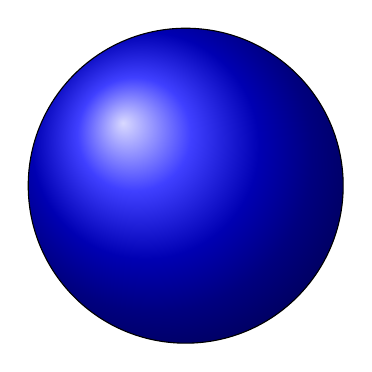
\begin{tikzpicture}
          \draw[shading = ball] (0, 0) circle (2);
    \end{tikzpicture}
\end{document}
    \caption[One ball]{One ball.}
\end{figure}

% Standalone with \includegraphics:
\begin{figure}[thbp]
    \centering
    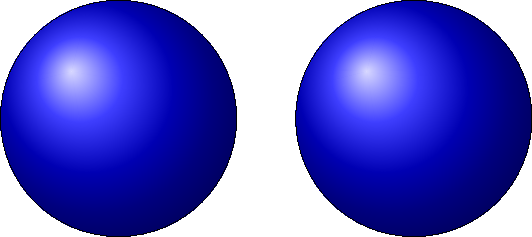
\includegraphics{balls}
    \caption[Two balls]{Two balls.}
\end{figure}

% Todonotes:
\begin{figure}[hbp]
    \centering
    \missingfigure{Three balls.}
    \caption[Three balls]{Three balls.}
\end{figure}

\kant[5-6] % Dummy text

% Booktabs:
\begin{table}[htbp]
    \centering
    \begin{tabular}{@{}ll@{}}
        \toprule
        \textbf{Correct}               & \textbf{Incorrect}      \\
        \midrule
        \( \varphi \colon X \to Y \)   & \( \varphi : X \to Y \) \\[0.5ex]
        \( \varphi(x) \coloneqq x^2 \) & \( \varphi(x) := x^2 \) \\
        \bottomrule
    \end{tabular}
    \caption[Colons]{Proper colon usage.}
\end{table}

\begin{table}[htbp]
    \centering
    \begin{tabular}{@{}ll@{}}
        \toprule
        \textbf{Correct}     & \textbf{Incorrect}         \\
        \midrule
        \( A \implies B \)   & \( A \Rightarrow B \)      \\
        \( A \impliedby B \) & \( A \Leftarrow B \)       \\
        \( A \iff B \)       & \( A \Leftrightarrow B \)  \\
        \bottomrule
    \end{tabular}
    \caption[Arrows]{Proper arrow usage.}
\end{table}

% Tablefootnote and multirow:
\begin{table}[htbp]
    \centering
    \begin{tabular}{@{}ll@{}}
        \toprule
        \textbf{Correct}
        & 
        \textbf{Incorrect}
        \\
        \midrule
        \( -1 \) 
        & 
        -1
        \\[0.3ex]
        1--10
        &
        1-10
        \\[0.3ex]
        Birch--Swinnerton-Dyer\tablefootnote{It is now easy to tell that Birch and Swinnerton-Dyer are two people.} conjecture
        &
        Birch-Swinnerton-Dyer conjecture
        \\[0.3ex]
        The ball \dash which is blue \dash is round.
        &
        \multirow{ 2}{*}{The ball - which is blue - is round.}
        \\[0.3ex]
        The ball---which is blue---is round. 
        &
        \\
        \bottomrule
    \end{tabular}
    \caption[Dashes]{Proper dash usage.}
\end{table}

\section{Outline}

The rest of the thesis is organised as follows:
\begin{description}
    \item[\cref{sec:second}]
    is second to none, with the notable exception of \cref{sec:intro}.
    The main tool introduced here is the employment of unintelligible sentences.
    
    \item[\cref{sec:third}]
    asserts the basic properties of being the third chapter of a thesis.
    This section reveals the shocking truth of filler content.
    
    \item[\cref{sec:fourth}]
    demonstrates how easily one can get to four chapters by simply using the \texttt{kantlipsum} package to generate dummy words.
    
    \item[\cref{sec:first-app}]
    features additional material for the specially interested.
    
    \item[\cref{sec:source}]
    consists of results best relegated to the back of the document,
    ensuring that nobody will ever read it.
\end{description}

    \chapter{Motion Planning}
\label{sec:MotionPlanning}

% Alternative outlay:
% Overview -> Representation (discrete, cont, determ, prob, state-space
% implici/explicit)

\section{Overview/Preliminaries}
Motion planning is the task of manipulating a robot's configurations so that,
given an initial and goal state or posture, the planner (black box), is able
to create a sequence of actions that gives a feasible or optimal path through
the overarching planning environment, usually referred to as the world space.
Thus a motion planner can be seen as a machine which given an the input: a
world, and initial and goal states, produces a sequence of actions to move the
robot from its initial to the desired goal configuration. This plan is then
passed on to the trajectory generator in the system. Generally, planners can be
separated into complete and non-complete planners, meaning that given enough
time, all motion planning problems are solvable, only the solution is NP-Hard.
Thus feasible solutions will have to make compromise, and a lot of planners in
use today are what is called probabilistically complete, meaning that they
converge to a solution given infinite time. As such time-frames are of no use to
us, we generally have to settle for an approximation bound. There is a
difference between online and off-line motion planning, whereas the offline
algorithm plans in a static environment, the online algorithm is run
continuously. However an online algorithm can be simulated by running an offline
algorithm repeatedly for short intervals of time. However, this comes with the
drawback, that no guarantee can be made for completing a certain task.

\subsection{Building Blocks}

\subsection{The Robot and World Model}

The modelled world \(\mathcal{W}\), and eveything in it can be modelled
geometrically using any number of methods -- most usually polygons or some other
convex gemoetric structure. Thus the robot can also be modelled as a collection
of gemoetric structures \(\mathcal{A}\). Thus in order to move the robot in the
world space, rigid body transformations are applied. Given the robot as a subset
of the world space, the image of a robot transformation is then given as:
% \[
%   h(\mathcal{A}) = \set{h(a) \in \mathcal{W} \mid a \in \mathcal{A}} \\
%   h \colon \mathcal{A} \rightarrow \mathcal{W} \\
%   \mathcal{A} \and h(\mathcal{A}) \subset \mathcal{W} \\
% \]

The world as we model it contains two kinds of objects

\begin{itemize}
\item \textbf{Robot:} Body that is modeled geometrically and is controllable via
  a motion plan.
\item \textbf{Obstacles:} Portions of the world that are occupied by something
  other than the robot.
\end{itemize}

\subsection{Rigid Transformations}
\label{sec:rigidtransformations}


% \subsection{State Space}
% \label{subsec:State}
% Planning problems involve a state space. A state space is a set of all the
% possible configurations a model can be in at any given time. The state space can
% be either discrete or continuous, and can be represented either implicitly or
% explicitly.

\subsubsection{Configuration Space}
\label{sec:configuration-space}
The configuration space is a general abstraction used as a model for a wide
variety of motion planning problems. It is a manifold that arise from the
transformations applied to the robot. If the robot has n-degrees of freedom, the
set of transformations is usually a manifold of dimension n. This manifold is
called the configuration space of the robot, and is shortened \(\mathcal{C}\).
Thus in order to solve a motion planning problem, a search must be performed in
the configuration space. Thus the motion planning problem is now made into a
question of finding the best path to traverse the given manifold\cite{Lav06}. (characterize and describe the
configuration space structure.)
In our case the configuration space can be modeled as a topological space of
the type \(SE(3)\), meaning special-Euclidean three.

Using generalized coordinates, the configuration of a robot can be modeled as a
vector with n variables for the position in the configuration space, in
literature this space is usually denoted by \(\mathcal{C}\). As is most common,
the robot is modeled as a rigid body, in which two bodies cannot overlap, thus
points in the configuration space is separated into two sets. One set for which
the robot configuration overlaps with another object in the configuration space,
and is called \(\mathcal{C}_{Obst}\), and given that the world space is
represented as \(\mathcal{W}\), the collision free space is the given as
,\(\mathcal{C}_{free} = \mathcal{W}\setminus \mathcal{C}_{Obst}\). The
obstacle space can be represented in a number of ways, but we will stick to
polygonal models of the obstacle space.

\subsection{Action Space}
The action space is the set of actions that can be applied at any given state
the robot is located in. Thus one can model the action space as a function of
the robot's state. e.g.
\[
  U(x) = \set{u \in U \mid U(x) \neq \emptyset }
\]

\subsection{Initial and Goal States}
It is normal to define an initial state and a goal state as a starting and an
ending point of a planning problem. Where both the initial, and goal states can
be sets of states, meaning that it is not necessary to arrive specifically at
the target point. A starting point consisting of multiple configuration states
usually infers some kind of uncertainty in the robot model. The end goal can be
reached in one of two ways, wherein the two types characterize two different
forms of planning.
\begin{enumerate}
\item\textbf{Feasible:} Feasible planning has no concerns with optimality, and
  only concerns itself with finding a plan that arrives at the goal state.
\item\textbf{Optimal:} Optimal planning optimizes a feasible plan in some
  specified manner, with respect to some specified cost function.
\end{enumerate}

\subsection{A Plan}
If we are dealing with a fully deterministic model, a plan can simply be the set
of actions applied at each state in order to reach a goal state specified for
the problem at hand. However, if some measure of uncertainty is added to the
model, then literature describes this as planning in the \textit{information
  space}, and future states cannot be predicted exactly, thus some kind of
feedback model is used in order to plan in an uncertain environment. If we are
merely looking at solving the problem, a feasible plan is good enough, which
means a solution has to be found, but multiple solutions do not have to be found
and compared. However, if time, energy or some other parameters are to be
optimized, then a cost function has to be added into the planning model, in
order to evaluate which plan scores best when measured up against the others.

\subsection{Model}

\subsubsection{Discrete}
let \(\mathcal{X}\) be the discrete state space, and \(\ mathcal{U}(x)\) be
the set of actions available at each point \(x \in \mathcal{X}\).
state transition:
\[
  x_{k+1} = f(x_k, u_k)
\]

\subsubsection{Continuous}

\subsubsection{Path and Trajectory}

The motion plan takes the form of a path, or a trajectory. This is represented
as a function \(\phi(\alpha) \colon [0,1] \rightarrow \mathcal{X}\), where
\(\mathcal{X}\) is the configuration space of the vehichle. If the
control-execution time is considered, then the explicit model of vehicle
kinematics and/or dynamics, as well as the dynamics of the possible obstacles.
Then the trajectory is represented as a time-parametrized function of the kind
\(\pi(t) \colon [0,T] \rightarrow \mathcal{X}\), where \(T\) is the planning
horizon. Unlike the path, the trajectory describes how the configuration of the
vehicle evolves over time.

Initial and Goal States. A path is a function f \ldots

\subsection{Time}
\label{subsec:Time}

Discrete vs Continuous

\subsection{Actions}
\label{subsec:Actions}

A plan is a sequence of actions that manipulate the state of the robot.

A planning problem involves a sequence of decisions made over time.


car-like model can look something like:

\section{Algorithms}
In general there are algorithms for which every motion planning problem can be
solved explicitly, only their running time is on the order of \(O(!n)\) , and thus
not feasible in practical applications. In the practical case it is therefore
normal to employ methods of approximation.

\subsection{Grid-based Search}
\hyphenation{grid-based-search}
\label{subsec:gridbasedsearch}

\subsection{Interval-based Search}
\hyphenation{interval-bases-search}
\label{subsec:intervalbasedsearch}

\subsection{Geometric Algorithms}
\hyphenation{geometric-algorithms}
\label{subsec:geometricalgorithms}

\subsection{Artificial Potential Fields}
\hyphenation{artificial-potential-fields}
\label{subsec:artificialpotentialfields}

\subsection{Sampling-based}
\label{subsec:samplingbased}









\section{Piano Mover's Problem}

\section{Discrete vs Continuous}

\section{Sampling}

\section{State Space}

\section{Complexity}

\section{Criterions}

\subsection{Feasibility}
\subsection{Optimality}

\section{Completeness}

\section{Probabilistic Completeness}

\section{Planning Under Uncertainty (Decision Theoretic Planning)}

All real life motion planning problems are faced with some level of uncertainty,
as errors can arise from a multiple of sources, whereas the most prevalent ones
are uncertainty in:
\begin{enumerate}
\item motion
\item sensing
\item the environment
\end{enumerate}
Thus the exact system state is never exactly known. Therefore planning under
uncertainty is done in a belief space. Which is a description of the state space
using probability distributions. (Partial observability?)
Planning is done in the information space, as opposed to the state-space.
Uncertainties in prediction and the current state exist.
Forward and backward projections.

(probability constraint violation)

\subsection{A Game Against Nature}

Theta is nature's actions. U is the robot's action.

\subsection{A Model of Uncertainty}

If the discrete state space model is expanded to include \(\ Theta\) as the
space of nature actions, and \(\ theta_k\) is the action selected by nature at
step k, then a transition is modeled as
\[
  x_{k+1} = f(x_k,u_k,\theta_k)
\]
As the actions of nature are not available beforehand, that is - \(\theta_ k\) is
not given, thus we have
\[
  X_{k+1} =  \set{ x_{k+1} \ in X \mid \exists\theta_k \in \Theta(x_k,u_k)
    \text{ such that }
    x_{k+1} = f(x_k,u_k,\theta_k)}
\]
\cite{Lav06}.

\subsection{Discrete Planning with Nature}
a model of discrete planning with nature: \cite[pg,496]{Lav06}

A markov decision process is defined in \cite[pg.498]{Lav06} as:
\begin{enumerate}
\item A non empty \textit{state space} \(X\) which is a finite or countably
  finite set of \textit{states}.
\item For each state, \(x \in X\), a finite non-empty \textit{action space}
  \(U(x)\). It is assumed that \(U\) contains a special \textit{termination
    action}, which has the same effect as (cite the deterministic discrete
  planning model).
\item A finite non-empty \textit{nature action space} \(\Theta(x,u)\) for each
  \(x \in X\) and \(u \in U\).
\item A state transition function \(f\) that produces a state,
  \(f(x,u,\theta)\), for every \(x \in X\), \(u \in U\), and \(\theta \in
  \Theta\).
\item A set of \textit{stages}, each denoted by k, that begins at k=1 and
  continues indefinitely. Alternatively, there may be a fixed maximum stage \(k
  = K+1=F\).
\item An \textit{initial state} \(x \in X\). For some problems, this may not be
  specified, in which case a solution plan must be found from all initial
  states.

\item A \textit{goal set} \(X_G \subset X\).
\item A stage-additive cost functional L. Let \(\sim{\theta}_K\) denote the
  history of nature actions up to stage K. The cost functional may be applied to
  any combination of state, action, and nature histories to yield
  \[
    L(\sim{x}_F, \sim{u}_K, \sim{\theta}_K) = \sum_{k=1}^{K} l(x_k,u_k,\theta_k)
    + l_F(x_F)
  \]
  in which \(F = K + 1\). The termination action \(u_T\) is applied at some
  stage k, then for all \(i \geq k\), \(u_i = u_T\), \(x_i = x_k\), and
  \(l(x_i,u_T, \theta_i) = 0\).
\end{enumerate}
\cite[pg 498]{Lav06}

using this formulation either a feasible or optimal planning problem can be formulated.

\subsection{Forward and Back-Projections (under uncertainty)}

\subsection{Separating a plan from its execution}

\subsection{Feedback}

\subsection{Information Space}
A stochastic environment.
The information space is a general structure for working with plans under
conditions of uncertainty. Thus planning can be done mostly as it is done in a
state space, albeit in a higher dimension. Thus the state transition function
can be written as
\[
  \phi_{k+1} = f_{\mathcal{I}}\left( \phi_k, \mu_k, y_{k+1} \right)
\]

\subsection{Nondeterministic and Probabilistic Information Spaces}

\subsection{A Plan under Uncertainty}
Since it
Expected-case analysis. Worst-case analysis.

Uncertainty comes from three sources in our model:
\begin{enumerate}
\item The Model (motion).
\item The observation (sensor).
\item The environment (map).
  Grid-based problems: Navigation: A goal position is to be reached, even though
  the map is unknown. The robot is allowed to solve the problem without fully
  exploring the environment. Only a part of the environment is needed to solve
  the problem.
  Searching: A goal state can only be identified when it is reached by a
  short-range sensor. The environment is systematically searched, but the search
  may terminate early if the goal is found.

  Problem-definition:
  Part of the problem is map-building, as the map is not provided exactly, and
  sensory map-information has to be used in order to successfully solve a given
  planning problem.
\end{enumerate}

\subsection{Visibility Polygon}
Let \(V(x)\) be the visibility polygon - that is the set of all points that are
visible from \(x\).

I-states enables us to solve problems without having a complete represenation of
the environment! (LAV06)chp12.2



\subsubsection{Decision Makers}

\subsection{Rewards?}

\section{Data Collection and Sensors}



\section{Optimality}



\section{Survey of Papers}

\subsection{Related Work}

http://msl.cs.uiuc.edu/~lavalle/cs497/jokane.pdf

http://robotics.cs.unc.edu/BeliefSpacePlanning/index.html

\section{Survey}

Following is a survey of motion planning techniques with a focus on their
application in unmanned ground vehichles (UGVs). First described is the relevant
sources of uncertainty in UGV motion planning, and then describes the relevant
techniques that have been applied to solve them in the literature. In general
uncertainty in UGV planning can be related to three sources:
\begin{enumerate}
\item Uncertainty in robot sensing.
\item Uncertainty in robot predicability.
\item Uncertainty in environment sensing.
\item Uncertainty in environment predicability.
\end{enumerate}
\cite{lavalle_framework_1995}

\subsection{Uncertainty in robot predicability}
Uncertainty in vehicle dynamics arises as the future robot configuration cannot
be predicted exactly. This results from modelling errors and/or limited
precision in the system's command tracking performance
\cite{dadkhah_survey_2012}. Thus a transfer from one state to another will not
guarantee full knowledge of the vehichle in the next state. This is referred to
as \textit{automated sequential decision making} in the literature, and the
mathematical framework used to tackle such uncertainty is the \textit{Markov
  Decision Process} (MDPs), used to formulate an optimal value problem, which
then can be solved for an optimal value function, and the corresponding optimal
policy \cite{Cassandra:1998:EAA:926710}. The problem herein lies with the size
of the state space when this solution strategy is applied to solving real-world
problems -- referred to as \textit{the curse of dimensionality}. In fact
\cite[Tsilkis]{christos_h._papadimitriou_complexity_1987} showed that solving
such a problem is PSPACE-Complete and thus not tractable for real-life
applications. However approximate solutions are available, as shown by
\cite[Kaelbling et. al]{kaelbling_planning_1998}. Therefore the problem has to
be solved by using techniques such as sampling the belief space, as shown in
\cite[Kearns et. al]{kearns_sparse}.

% \subsubsection{Optimal Control Based Approaches}

\subsection{Uncertainty in Environment Predicability}
If the robot has imperfect or non-existent a-priori maps, or noisy sensory data,
complete deterministic knowledge of the environment is impossible.

\subsubsection{Planning techniques for an uncertain environment} 
For an UGV in an unknown environment, being able to have the situational
awareness to avoid collisions while adhering to the global planning
requirements, despite unpredicted obstacles appearing, is essential. Thus
environment sensing and mapping and re-planning in real-time is required. This
is referred to in the literature as planning in partially unknown environments.
One solution to this problem is through incremental graph-search algorithms, as
shown in \cite[Stentz]{stentz_optimal}, where the \textsl{D*} algorithm is
described as a method for optimal and efficient replanning in partially unknown
environments. Then \textit{Stentz}, a year later published the \textit{Focused
  D*} algorithm a year later \cite{stentz1995focussed}, which incorporates
heuristics to reduce the total time taken for re-planning. Still,\textit{D*} is computationally heavy, and algorithms have
been created to improve on the time-bound of \textit{D*}. One notable is the
\textit{D*-lite} algorithm presented by \cite[Koenig]{koenig2002d}. These
incremental planners, which incorporates the previously calculated plan in the
solution of the newly arisen planning problem speeds up the planning cycles, but
can in many cases still not be enough for a viable real-time solution. Finding a
new plan within the allotted planning interval may simply not be possible, in
which case one can resort to \textit{Anytime} algorithms, like \cite[Karaman et.
al]{karaman_anytime_2011}, or one can



    \part{The First Part}

    % \chapter{The Planner}
\label{sec:planner}


\section{The Planning Algorithm}

\subsection{RRT}

The RRT algorithm is a sampling based algorithm which \ldots

\kant[7-11] % Dummy text

    % \chapter{Model}

\section{Kinematic Model Description}

\section{Dynamic Model Description}

The kinematics and dynamics are based on the paper: http://www.cs.cmu.edu/~motionplanning/reading/PlanningforDynamicVeh-1.pdf.

The optimisation objective?

The optimisation heuristics?


    % \chapter{The Second Chapter}
\label{sec:second}

\kant[7-11] % Dummy text

\begin{theorem}[{\cite[95]{AM69}}]
    \label{thm:dedekind}
    Let \( A \) be a Noetherian domain of dimension one. Then the following are equivalent:
    \begin{enumerate}
        \item \( A \) is integrally closed;
        \item Every primary ideal in \( A \) is a prime power;
        \item Every local ring \( A_\mathfrak{p} \) \( (\mathfrak{p} \neq 0) \) is a discrete valuation ring.
    \end{enumerate}
\end{theorem}
    % \chapter{The Third Chapter}
\label{sec:third}
\kant[12-13] % Dummy text
\section{First Section}
\kant[14]    % Dummy text
\section{Second Section}
\kant[15]    % Dummy text
    % \chapter{The Fourth Chapter}
\label{sec:fourth}
\kant[15-19] % Dummy text

    % \appendix           % "Chapter" is renamed "Appendix"
    % \appendixpage       % Similar to \part*{Appendices}, but appears in TOC.

    % \chapter{The First Appendix}
\label{sec:first-app}
\kant[20-21] % Dummy text
\section{First Section}
\kant[22]    % Dummy text
\section{Second Section}
\kant[23-24] % Dummy text
    % \chapter{Source Code}
\label{sec:source}
\section{Implementation}
The \texttt{phduio} class is implemented in the following way:
\lstinputlisting[language = {[LaTeX]{TeX}}]{phduio.cls}

    \backmatter         % Folios in Arabic numerals, unnumbered chapters.

    \printbibliography

\end{document}
